\documentclass{article}
\usepackage{graphicx} % Required for inserting images
\usepackage{booktabs}
\usepackage{amsmath}
\usepackage{amssymb}
\usepackage{float} % [H] placement: keep figures and tables where they appear in the source

\title{Portfolio 1: A Double Bongcloud Analysis}
\author{Michael Robinette}
\date{September 2026}

\begin{document}

\maketitle

\section*{Data construction and description}
We leverage lichess game data from March 2021 (~100 million games), which can be downloaded from https://database.lichess.org/. The initial download was 229.34 GB and contained the fields seen in Table~\ref{tab:pgn-fields}. We extract rated blitz games that open 1.e4 e5 2.Ke2 (5,068 games) and record the fields in Table~\ref{tab:extracted-fields}. The double bongcloud subset is the 324 games with \texttt{bke7} $= 1$. To verify extraction, we compare to lichess's history API endpoint, which records 323 games, whcih reach the double bongcloud.

\begin{table}[H]
\centering
\caption{Game record fields in the Lichess standard rated PGN export.}
\label{tab:pgn-fields}
\begin{tabular}{ll}
\toprule
\textbf{Field} & \textbf{Type} \\
\midrule
\texttt{Event}           & String (categorical: speed, plus tournament URL when applicable) \\
\texttt{Site}            & String (URL; unique game identifier) \\
\texttt{Date}            & Date (\texttt{YYYY.MM.DD}) \\
\texttt{Round}           & String (constant \texttt{-}) \\
\texttt{White}           & String (username) \\
\texttt{Black}           & String (username) \\
\texttt{Result}          & Categorical (\texttt{1-0}, \texttt{0-1}, \texttt{1/2-1/2}, \texttt{*}) \\
\texttt{UTCDate}         & Date (\texttt{YYYY.MM.DD}) \\
\texttt{UTCTime}         & Time (\texttt{HH:MM:SS}, UTC) \\
\texttt{WhiteElo}        & Integer (Elo rating) \\
\texttt{BlackElo}        & Integer (Elo rating) \\
\texttt{WhiteRatingDiff} & Signed integer (Elo points gained or lost) \\
\texttt{BlackRatingDiff} & Signed integer (Elo points gained or lost) \\
\texttt{WhiteTitle}      & String (optional; federation title, e.g.\ \texttt{WFM}) \\
\texttt{ECO}             & String (ECO code, \texttt{A00}--\texttt{E99}, or \texttt{?}) \\
\texttt{Opening}         & String (opening name, or \texttt{?}) \\
\texttt{TimeControl}     & String (\texttt{base+increment}, in seconds) \\
\texttt{Termination}     & Categorical (\texttt{Normal}, \texttt{Time forfeit}, \texttt{Abandoned}) \\
\texttt{Movetext}        & String (SAN moves with inline clock comments) \\
\bottomrule
\end{tabular}
\end{table}

\begin{table}[H]
\centering
\caption{Fields of the extracted dataset and their role in filtering for the double bongcloud.
All 5{,}068 extracted games have \texttt{e4e5} $=$ \texttt{wke2} $= 1$; filtering on \texttt{bke7} $= 1$ leaves 324 games.}
\label{tab:extracted-fields}
\begin{tabular}{llp{6.5cm}}
\toprule
\textbf{Field} & \textbf{Type} & \textbf{Description} \\
\midrule
\texttt{date}      & Date    & Game date, from \texttt{UTCDate} \\
\texttt{white}     & String  & White's username \\
\texttt{white\_elo} & Integer & White's blitz rating at the start of the game \\
\texttt{black}     & String  & Black's username \\
\texttt{black\_elo} & Integer & Black's blitz rating at the start of the game; \textbf{the modeled outcome} \\
\texttt{e4e5}      & Binary  & 1 if the game opened 1.e4 e5 \\
\texttt{wke2}      & Binary  & 1 if White played 2.Ke2 (the Bongcloud Attack) \\
\texttt{bke7}      & Binary  & 1 if Black replied 2\ldots Ke7 (the double bongcloud); \textbf{filter for the modeled subset} \\
\texttt{opening}   & String  & Lichess's own opening name, from \texttt{Opening}; used to cross-check the move scan \\
\texttt{moves}     & String  & Full move sequence in SAN, from the movetext \\
\bottomrule
\end{tabular}
\end{table}

\section*{Modeling question}
Question: 
Because Bongcloud Attack invokes an immediate violation of key chess principles, it is considered to be a joke or meme opening. In March of 2021 Magnus Carlsen, the highest rated chess player in the world played it against Hikaru Nakamura, considered to be the second best player in the world. As a result the joke took off as we see in Figure~\ref{fig:bongcloud_games}. In light of this phenomenon, examine the response to the Bongcloud Attack. Specifically we examine the mean elo of the player that gets the joke and responds with the Double Bongcloud Attack.
\begin{figure}[H]
\centering
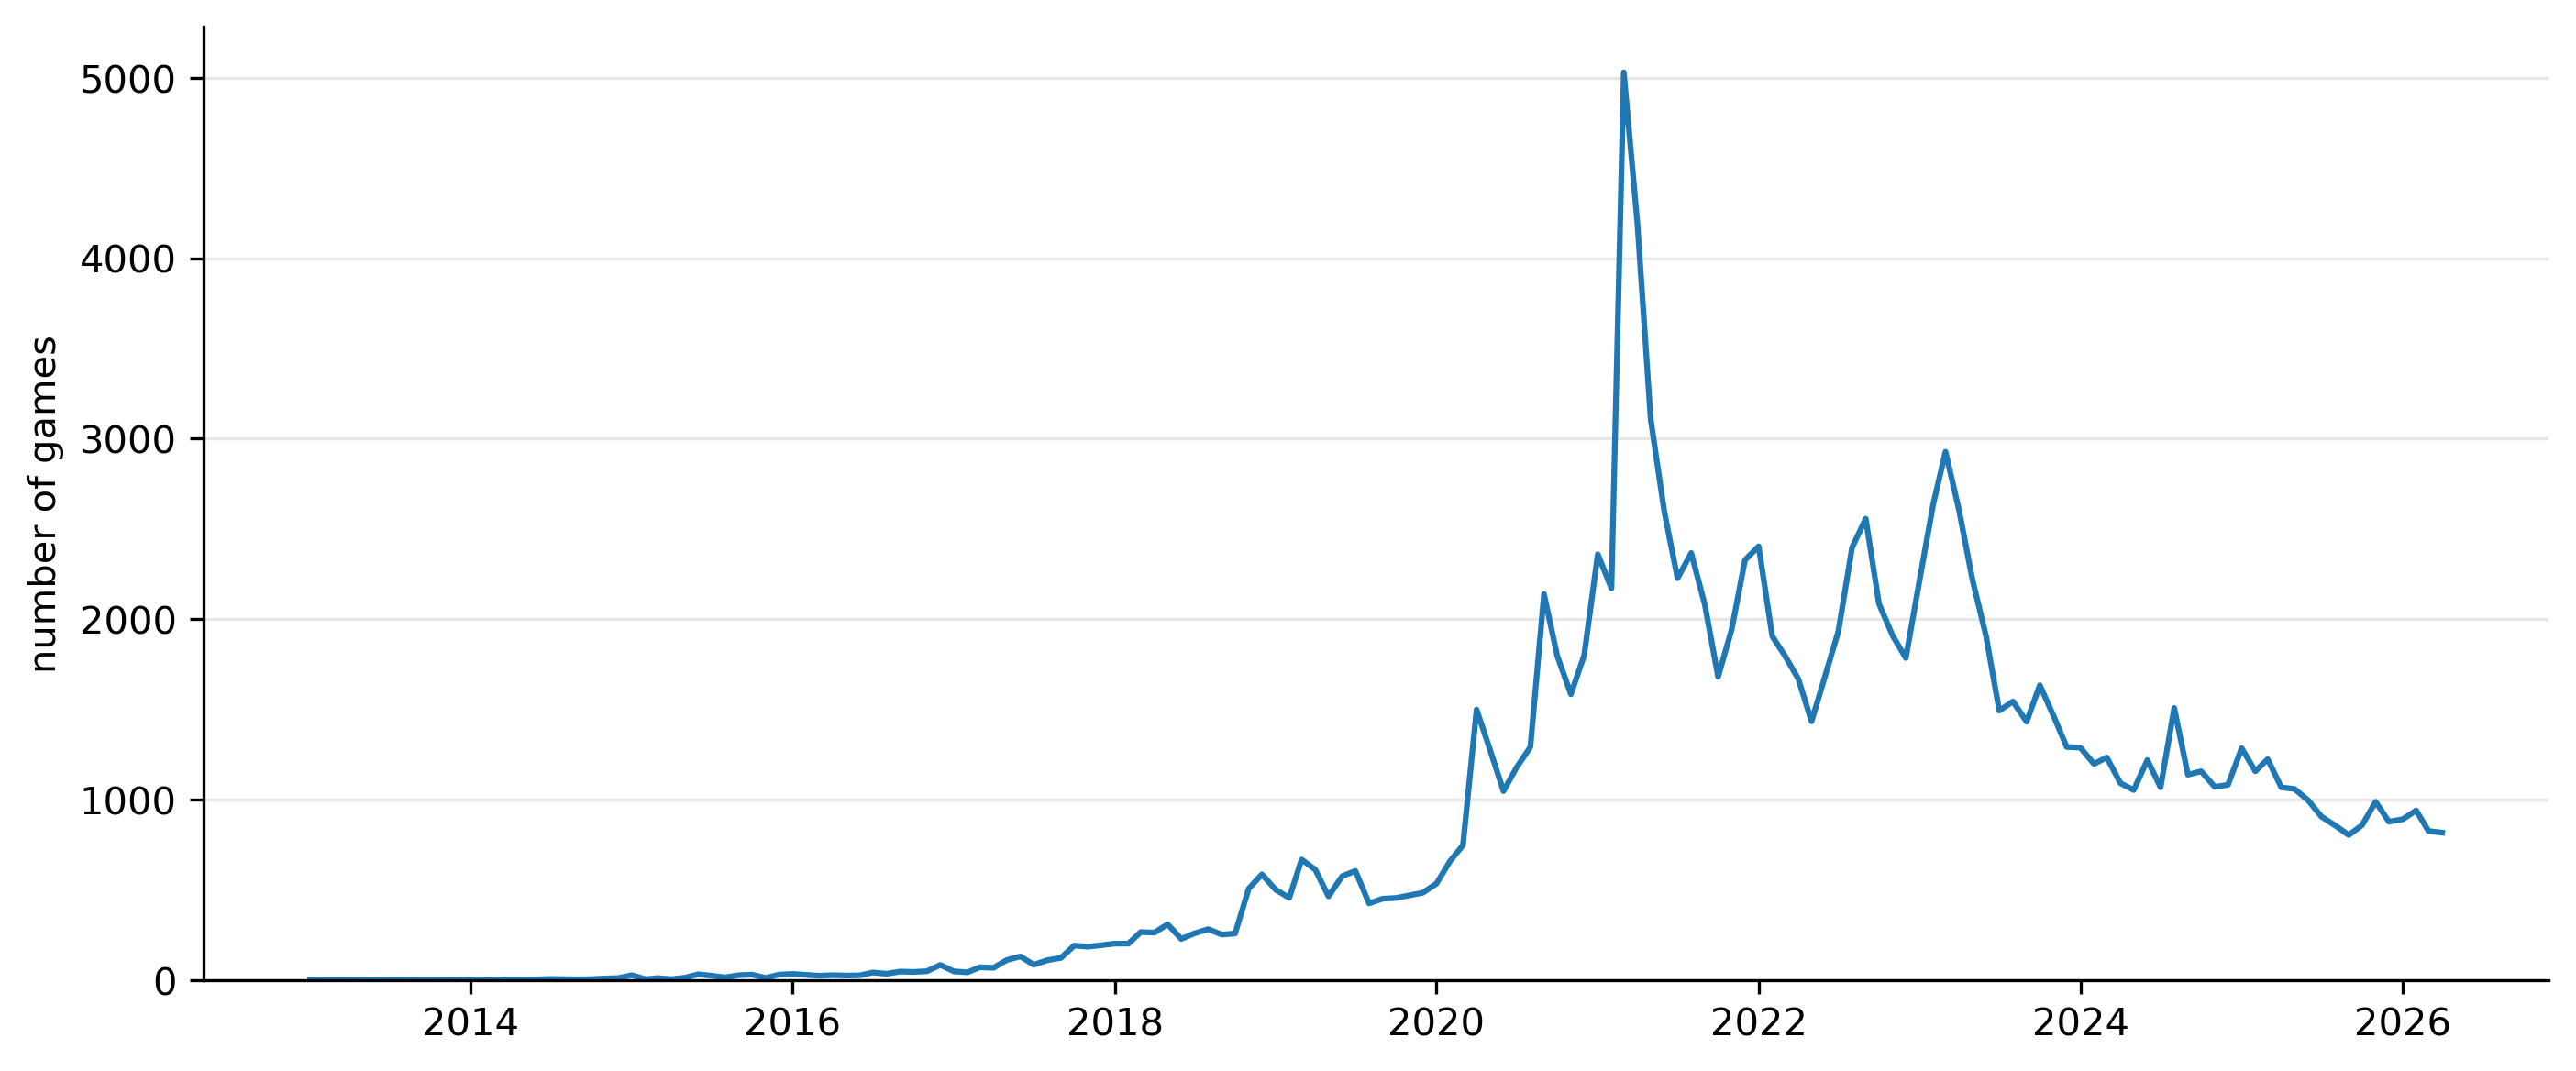
\includegraphics[width=0.75\linewidth]{figures/bongcloud_games.png}
    \caption{\textbf{Games reaching 1.e4 e5 2.Ke2, by month.}}
\label{fig:bongcloud_games}
\end{figure}
\section*{Model description}
\begin{align*}
y_i \mid \mu, \sigma &\overset{\text{ind.}}{\sim} \mathrm{Normal}(\mu, \sigma), \qquad i = 1, \dots, N,\\
\mu &\sim \mathrm{Normal}(1500, 300),\\
\sigma &\sim \mathrm{Normal}^{+}(0, 400),
\end{align*}
where $\mathrm{Normal}^{+}$ is a normal distribution truncated below at zero,
and the second argument of each normal is a standard deviation, as in Stan.

\paragraph{In words.} Players who answer the Bongcloud Attack with 2\ldots Ke7 come from a population
whose blitz ratings are centered on an unknown mean $\mu$ and spread with an unknown standard
deviation $\sigma$. Each of the $N$ games gives an independent draw $y_i$ of Black's rating from
that population. Before seeing the data, we believe $\mu$ is most likely near Lichess's 1500
starting rating, and that $\sigma$ is positive and probably no larger than a few hundred points.

\begin{table}[H]
\centering
\caption{Quantities in the model.}
\label{tab:model-quantities}
\begin{tabular}{lllp{5cm}}
\toprule
\textbf{Symbol} & \textbf{Role} & \textbf{Support} & \textbf{Meaning} \\
\midrule
$y_i$      & Observed  & $\mathbb{R}$ (model); integers $\geq 600$ (reality) & Black's blitz rating in game $i$ \\
$N$        & Fixed     & $\mathbb{Z}^{+}$ ($N = 324$) & Number of double bongcloud games \\
$\mu$      & Parameter & $\mathbb{R}$     & Mean rating of double bongcloud responders \\
$\sigma$   & Parameter & $(0, \infty)$    & Spread of their ratings \\
1500, 300  & Fixed     & ---              & Prior mean and SD of $\mu$ \\
400        & Fixed     & ---              & Prior scale of $\sigma$ \\
\bottomrule
\end{tabular}
\end{table}

\paragraph{Why these distributions.}
\begin{itemize}
  \item \textbf{Normal likelihood.} A rating is a running total of many small wins and losses, so across
        players ratings are roughly bell-shaped around a typical value, and the observed histogram
        is unimodal. The Normal's two parameters map directly onto the modeling question: a typical
        rating ($\mu$) and how much players vary ($\sigma$). Its limitation is support: the Normal
        allows any real number, while Lichess ratings are integers that cannot fall below 600. With
        $\mu \approx 1300$ and $\sigma \approx 360$, only a few percent of the probability lies below 600, so we
        accept the approximation and test it in the posterior predictive check.
  \item \textbf{Normal prior on $\mu$.} $\mu$ can in principle take any real value, and a normal prior
        expresses a best guess (1500, the rating new accounts start at) with symmetric uncertainty.
        An SD of 300 allows group means from about 900 to 2100.
  \item \textbf{Half-normal prior on $\sigma$.} A standard deviation must be positive, so we truncate the
        normal at zero. A scale of 400 puts most prior mass below about 800, consistent with blitz
        ratings spanning roughly 600--3000.
  \item \textbf{Independence.} We assume games are independent given $\mu$ and $\sigma$. This is
        approximately true: there are 311 distinct Black players in 324 games, so only a few players
        contribute more than once.
\end{itemize}

\section*{Prior-predictive analysis}

\begin{figure}[H]
\centering
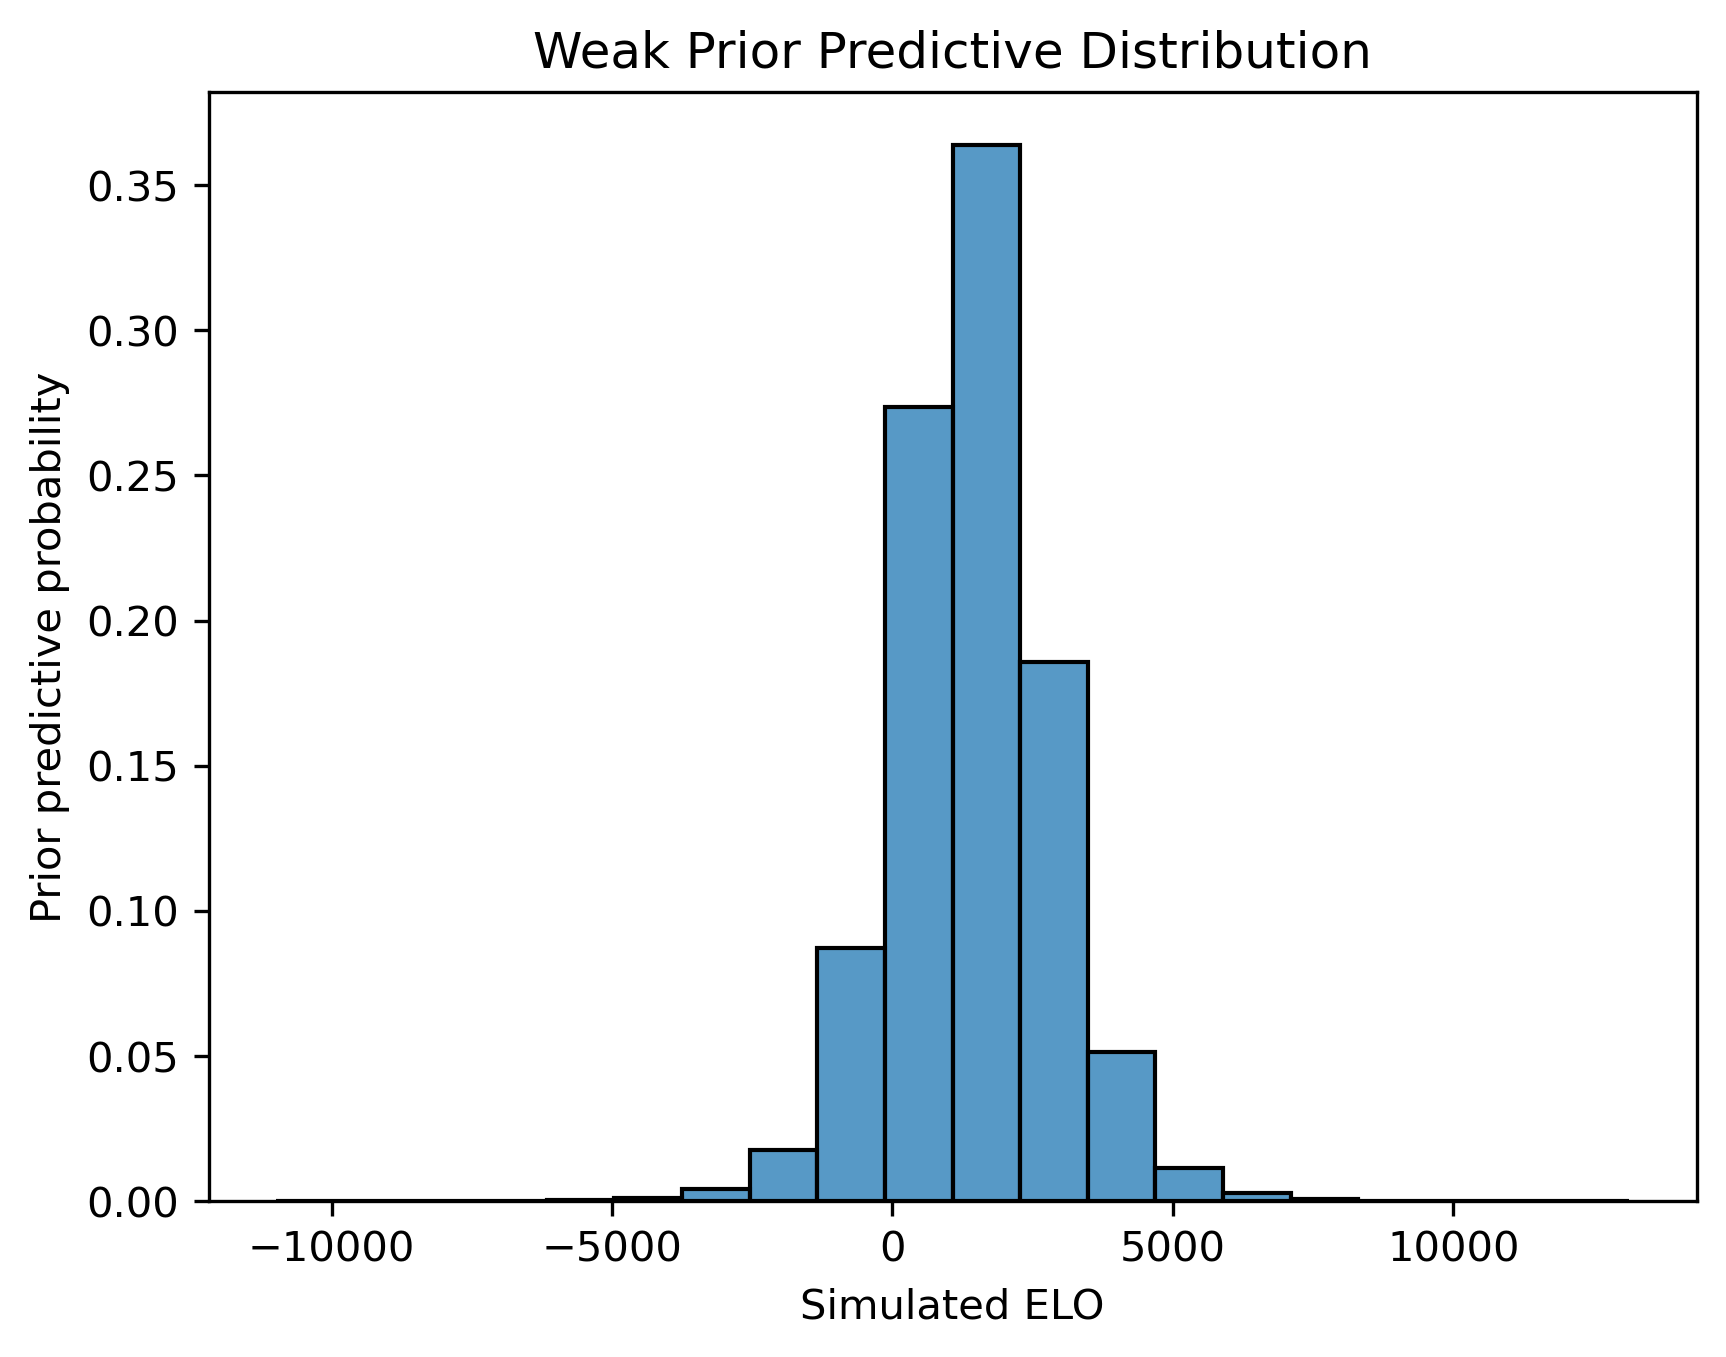
\includegraphics[width=0.75\linewidth]{figures/weak_prior_predictive.png}
\caption{\textbf{Weak Prior Predictive Distribution.} This figure was produced with the priors
$\mu \sim \mathrm{Normal}(1500, 1000)$ and $\sigma \sim \mathrm{Normal}^{+}(0, 1000)$. The broad prior produces impossible numbers. Notably we observe 13\% of values below 0 and 7\% of values above 3400.}
\label{fig:weak_prior_predictive}
\end{figure}
\section*{Estimation}
\section*{Posterior predictive check}
\section*{Interpretation}
\section*{Self-assessment}
\end{document}
